\documentclass{article}

\usepackage[T1]{fontenc}
\usepackage{polski}
\usepackage[utf8]{inputenc}

\usepackage{hyperref}
\usepackage[legalpaper, margin=1.2in]{geometry}

\usepackage{listings}
\usepackage[]{algorithm2e}

\title{AEM - Zadanie nr 4}
\author{Bartosz Sobkowiak 125342 Joanna Świda 138675}
\date{10.05.2020}

\usepackage{natbib}
\usepackage{graphicx}

\begin{document}

\maketitle
\section{Opis zadania}

    Rozważany problem to zmodyfikowana wersja problemu komiwojażera. Dany jest zbiór wierzchołków i macierz symetrycznych odległości między nimi. Zadanie polega na implementacji trzech metod - multiple start local search oraz dwóch rodzajów iterated local search.

\section{Pseudokod}

Wybraliśmy przeszukiwanie typu steepest, gdyż dawało najlepsze wyniki. \\
Używaliśmy wersji z zadania nr 2, czyli bez usprawnień.

\vspace{10mm}

\begin{algorithm}[H]
     \KwData{zbiór wierchołków, macierz odległości pomiędzy wierzchołkami}
     \KwResult{najlepsze rozwiązanie}
     
    wygeneruj losowe rozwiązanie S\\
    wyznacz elementy (wierzchołki) które nie znajdują się w rozwiązaniu \\
    \While{dopóki nie przekroczono czasu}{
        \textit{perturbate()} - wykonaj niewielką perturbację na rozwiązaniu S: \\
            czyli wylosuj X punktów do zamiany, zamień te z rozwiązania z losowymi spoza rozwiązania \\
            \textit{// optymalne X zostało ustawione na wartość X=20} \\
            
        wykonaj \textit{LocalSearch} (z zadania 2) na rozwiązaniu S po wprowadzonych zmianach \\
        \textbf{IF:} jeśli rozwiązanie po wprowadzonych zmianach jest lepsze - zapisz jako najlepsze znalezione do tej pory rozwiązanie
            }
            \textbf{return:} najlepsze rozwiązanie \\ \\
            
            
\caption{Iterated Local Search 1}
\end{algorithm}

\vspace{10mm}

\begin{algorithm}[H]
     \KwData{zbiór wierchołków, macierz odległości pomiędzy wierzchołkami}
     \KwResult{najlepsze rozwiązanie}
     
    wygeneruj losowe rozwiązanie S\\
    wyznacz elementy (wierzchołki) które nie znajdują się w rozwiązaniu \\
    \While{dopóki nie przekroczono czasu}{
        \textit{perturbate()} - wykonaj niewielką perturbację na rozwiązaniu S: \\
            \textit{destroy()} - usuń Y\% punktów z rozwiązania \\
            \textit{repair()} - napraw rozwiązanie w sposób zachłanny \\
            \textit{// optymalne Y zostało ustawione na wartość Y=20\%} \\
            
        wykonaj \textit{LocalSearch} (z zadania 2) na rozwiązaniu S po wprowadzonych zmianach \\
        \textbf{IF:} jeśli rozwiązanie po wprowadzonych zmianach jest lepsze - zapisz jako najlepsze znalezione do tej pory rozwiązanie
            }
            \textbf{return:} najlepsze rozwiązanie \\ \\
            
            
\caption{Iterated Local Search 2 - Destroy-Repair}
\end{algorithm}

\newpage

MSLS bazuje na algorytmie z zadania 2 \\

\begin{algorithm}[H]
     \KwData{zbiór wierchołków, macierz odległości pomiędzy wierzchołkami}
     \KwResult{najlepsze rozwiązanie}
    \For{wykonaj 100 razy}{
        wygeneruj losowe rozwiązanie\\
        \While{dopóki znalezione rozwiązania są lepsze}{
            \For{dla każdej pary indeksów w zakresie 0-99 w losowej kolejności} {
                podmień krawędzie według indeksów \\
                oblicz deltę dla zamienionych krawędzi\\
                jeśli delta jest mniejsza od najlepszej jak dotąd znalezionej delty: przypisz nową wartość najlepszej delty, to podmień w obecnym rozwiązaniu
            }\EndFor        
            jeśli zmienione rozwiazanie jest lepsze: wybierz je jako najlepsze\\
                }
        dodaj do listy rozwiązań \\
        posortuj i wybierz najlepsze \\
        \textbf{IF:} najlepsze rozwiązanie z tej iteracji jest lepsze niż najlepsze do tej pory znalezione rozwiązanie - ustaw je jako najlepsze znalezione, kontynuuj
    }\EndFor
    \textbf{return:} najlepsze rozwiązanie \\ 
    
    
\caption{Multiple Start Local Search}
\end{algorithm}

\vspace{10mm}


\section{Wyniki obliczeń i wizualizacje}

\begin{table}[h!]
\centering
\begin{tabular}{ |c|c|c|c|c|c| } 
 \hline
 Zbiór & Wersja & Typ & Min & Avg & Max \\ 
  \hline
 kroA$_{200}$ & ILS & 1 & 15279 & 17071 & 18271  \\ 
  \hline
 kroA$_{200}$ & ILS & 2 & 14142 & 14814 & 15466 \\ 
 \hline
 kroA$_{200}$ & MSLS & - & 16013 & 16935 & 18800 \\
  \hline
 kroB$_{200}$ & ILS & 1 & 15867 & 17068 & 18062 \\ 
  \hline
 kroB$_{200}$ & ILS & 2 & 14639 & 15147 & 15687 \\ 
 \hline
 kroB$_{200}$ & MSLS & - & 16631 & 16947 & 18348 \\
 \hline
\end{tabular}
\caption{Wartości rozwiązań}
\end{table}

\begin{table}[h!]
\centering
\begin{tabular}{ |c|c|c|c|c|c| } 
 \hline
 Zbiór & Wersja & Typ & Min & Avg & Max \\ 
  \hline
 kroA$_{200}$ & ILS & 1 & 200.0444 & 200.0628 & 200.1011 \\
  \hline
 kroA$_{200}$ & ILS & 2 & 200.118 & 200.1526 & 200.2765 \\
 \hline
 kroA$_{200}$ & MSLS & - & 200.013 & 200.126 & 200.098 \\
  \hline
 kroB$_{200}$ & ILS & 1 & 200.0407 & 200.0598 & 200.1157 \\
  \hline
 kroB$_{200}$ & ILS & 2 & 200.003 & 200.0487 & 200.0996 \\
 \hline
 kroB$_{200}$ & MSLS & - & 200.1207 & 200.1581 & 200.1457 \\
 \hline
\end{tabular}
\caption{Czasy trwania}
\end{table}

Średni czas trwania dla wykonywania 1 iteracji (spośród 100) dla algorytmu LocalSearch wchodzącego w skład MSLS to ok. 2.001s. \\

\begin{figure}[h!]
  \centering
  \begin{minipage}[b]{0.8\textwidth}
    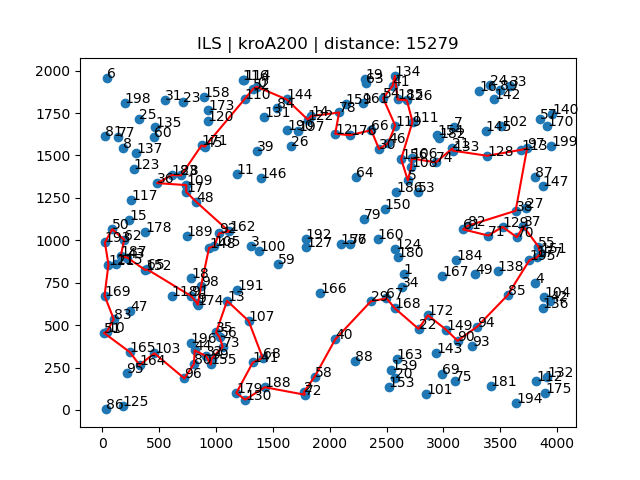
\includegraphics[width=\textwidth]{ils_kroA200.png}
  \end{minipage}

  \begin{minipage}[b]{0.8\textwidth}
    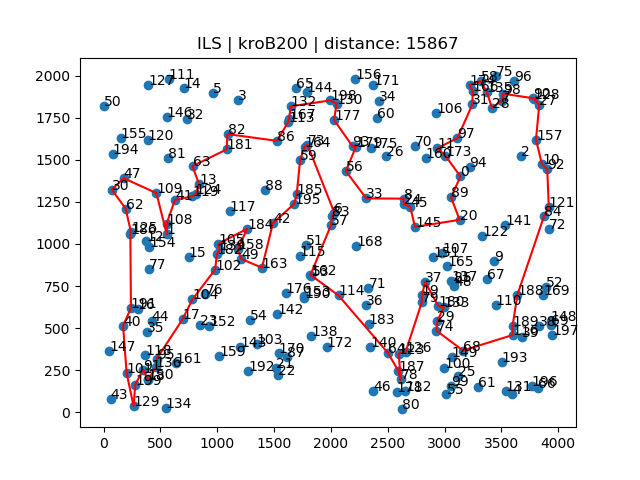
\includegraphics[width=\textwidth]{ils_kroB200.png}
  \end{minipage}
  
\end{figure}
    
\begin{figure}[h!]
    \centering
  \begin{minipage}[b]{0.8\textwidth}
    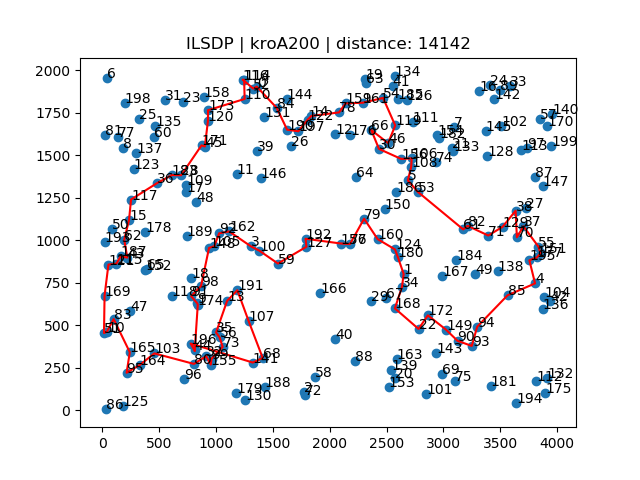
\includegraphics[width=\textwidth]{ilsdp_kroA200.png}
  \end{minipage}

  \begin{minipage}[b]{0.8\textwidth}
    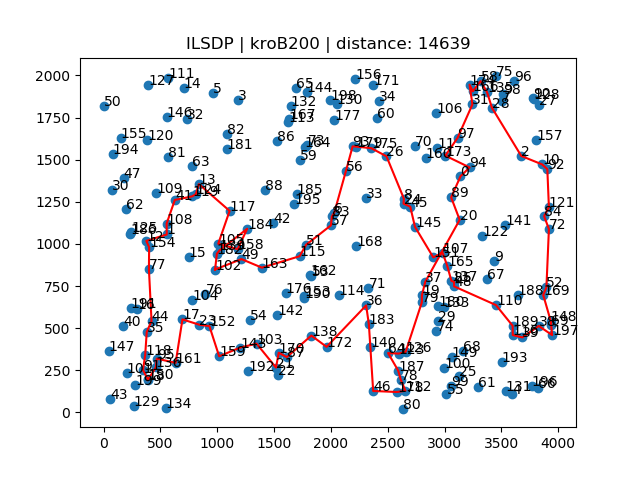
\includegraphics[width=\textwidth]{ilsdp_kroB200.png}
  \end{minipage}
\end{figure}

\begin{figure}[h!]
    \centering
  \begin{minipage}[b]{0.8\textwidth}
    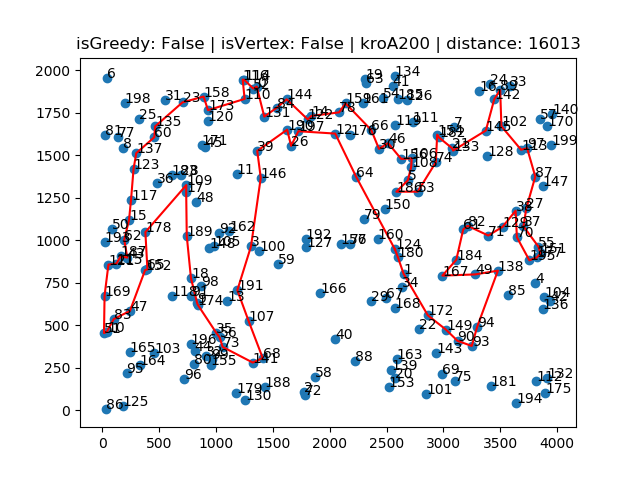
\includegraphics[width=\textwidth]{random_kroA200_V-False_G-False.png}
  \end{minipage}

  \begin{minipage}[b]{0.8\textwidth}
    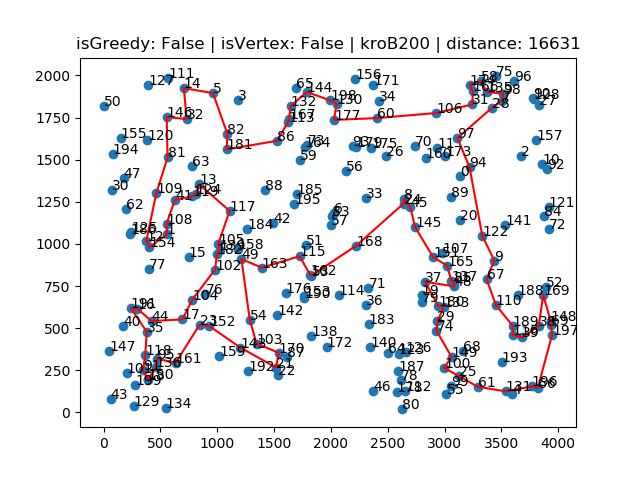
\includegraphics[width=\textwidth]{random_kroB200_V-False_G-False.png}
  \end{minipage}
\end{figure}


\section{Wnioski}

Z tabeli wyników można odczytać, że metody Iterated Local Seach dają lepsze wyniki niż metoda Multiple Start Local Search. Czas wykonywania po stronie ILS jest lepszy oczywiście dlatego, że w metodzie MLS zazwyczaj lokalnie przeszukujemy w pełni losowego rozwiązania. Jednakże w porównaniu do poprzednich metod czasy wykonywania zwiększyły się znacząco. Metoda ILS2 z naprawą rozwiązania okazała się nieco bardziej skuteczna od metody w której wymienialiśmy X wierzchołków. Prawdopodobnie wynikało to z tego, że w sposób losowy wymienialiśmy znaczącą liczbę wierzchołków - gdyby ta liczba była mniejsza (a procent "niszczonych" wierzchołków w ILS2 był większy), to wynik byłby odwrotny. Niemniej cel został osiągnięty, stosowanie metod ILS w tym przypadku jest lepszą metodą rozwiązania tego problemu.

\section{Kod programu}

    Repozytorium z kodem algorytmów dostępne jest pod: \url{https://github.com/bbbrtk/aem}


\end{document}
